%\customlink{Getting_a_paleomagnetic_direction}
\chapter{ Getting a paleomagnetic direction}

Rocks become magnetized in a variety
of ways (see Chapter 7).  Both igneous and sedimentary rocks can be affected by chemical
change, thereby acquiring a secondary magnetization.  Many magnetic materials are
affected by viscous remanent magnetization.  The various
components of magnetization sum together to constitute the 
NRM which is the ``raw'' remanence of the sample after extraction. 
The goal of paleomagnetic laboratory work is to isolate the various components
of remanence and to ascribe origin, age and reliability to these
components. But before the
laboratory work can begin, samples must be collected. Sampling
strategy is crucial to a successful study.  In this chapter, we will briefly describe techniques
for sampling, methods of orientation and
overall philosophy.  We will then turn to an overview of some of the more
 useful field and laboratory techniques that wind up with an estimate of a paleomagnetic direction.


\section {Paleomagnetic sampling}

\index{paleomagnetic!sampling}
There are several goals in paleomagnetic sampling:  one is to average out
the errors involved in the sampling process itself, and  to
assess the reliability of the recording medium (recording noise).  In addition, we
often wish  to  sample the range of  secular variation of the geomagnetic
 field in order to average it out or characterize its statistical properties.
The objectives of averaging recording and sampling
``noise'' are achieved by taking a number $N$ of individually oriented 
\index{paleomagnetic!sample}
{\it samples} from a
single unit 
\index{paleomagnetic!site}
(called a {\it site}).   Samples should be taken such that they represent a single time horizon, that is, they are from a single cooling unit or   the same sedimentary horizon. 
The most careful sample orientation procedure has an uncertainty of several degrees.
Precision is gained proportional to $\sqrt{N}$, so to improve the precision, multiple individually oriented samples are required.  The number of samples taken should be tailored to the
particular project at hand.  If one wishes to know polarity, perhaps three samples would be sufficient
(these would be taken primarily to assess recording noise). If, on
the other hand, one wished to make inferences about secular variation of
the geomagnetic field, more samples would be necessary to suppress sampling
noise.


Some applications in paleomagnetism require that  
the secular variation of the geomagnetic field (the paleomagnetic ``noise'')
be averaged in order to determine the
 time-averaged field direction.  The geomagnetic field varies with
time constants ranging from milliseconds to millions of years.  It is a
reasonable first order approximation to assume that, when averaged 
over, say,
10$^4$ or 10$^5$  years, the geomagnetic field is similar to that of  a geocentric axial dipole 
(equivalent to the field that would be produced by 
a bar magnet at the center of the Earth, aligned with the spin axis;
see Chapter 2).
Thus, when a time-averaged field direction 
is required, enough sites must be sampled
to span sufficient time to achieve this goal.  A general rule of thumb would be to aim for  about ten
sites (each with nine to ten samples), spanning 100,000 years.   If the distribution of  geomagnetic field vectors is desired, then more like 100 sites are necessary.  

\begin{figure}[h!tb]
%\epsfxsize 11cm
%\centering \epsffile {EPSfiles/drill.eps}
\centering  \includegraphics[width=11 cm]{EPSfiles/drill.eps}
\caption {Sampling technique with a water-cooled drill. [Photos of Daniel Staudigel.] a) Drill the
sample. b) Insert a non-magnetic slotted tube with an adjustable
 platform around the sample.  Rotate the slot to the upper side of the sample.
Note the azimuth and plunge of the drill direction (into the outcrop)
 with a sun and/or  magnetic compass 
and inclinometer.
 Mark the sample through the slot with a brass or copper wire.
c) Extract the sample.  d) Make a permanent arrow on the upper side of the
sample in the direction of
drilling and label the sample with the sample name. Make a note of the name
and orientation of the arrow in a field notebook. 
}
\label{fig:drill} 
\end{figure}


\begin{figure}[h!tb]
%\epsfxsize 11cm
%\centering \epsffile {EPSfiles/hand.eps }
\centering  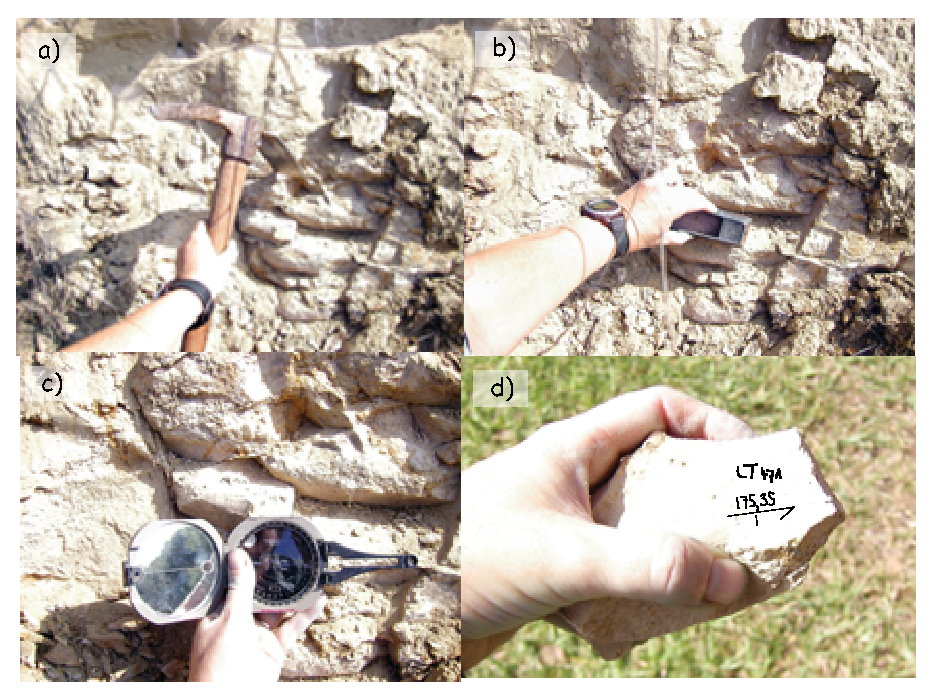
\includegraphics[width=11 cm]{EPSfiles/hand.eps}
\caption {Hand sampling technique for soft sediment:  a) Dig down to fresh material.  b)
Rasp off a flat surface. c) Mark the strike and dip on the sample. d)
Extract the sample and label it.}
\label{fig:hand}
\end{figure}


\subsection{Types of samples}

 Samples can be taken  using a gasoline or electric
powered drill,  as  ``hand samples'' (also known as ``block samples'' or as ``sub-samples'')  from a piston core.  

\begin{enumerate}  
\item {\it Samples cored with portable drill. }  The most common type of paleomagnetic sample is collected by
using a gasoline-powered portable drilling apparatus with a water-cooled diamond bit (Figure~\ref{fig:drill}a).
The diameter of cores is usually $\sim$2.5 cm. After drilling into the outcrop to a depth of 6 to 12 cm, 
an orientation device is slipped over the sample while it is still attached to the outcrop at its
base  (Figure~\ref{fig:drill}b and Figure~\ref{fig:orientation}).   Orientation devices have an inclinometer for determining dip (angle from the horizontal down or up) or the hade (angle from the vertical down direction)  of the
core axis.  They also have  a magnetic and/or sun compass  for determining azimuth of core axis. The accuracy
of orientation by such methods is about $\pm 3^{\circ}$. A fiducial mark is scratched on to the core with a brass wire (Figure~\ref{fig:drill}b), or if the core has broken free, a mark is made on the outcrop and transferred to the core (with a degradation of accuracy in orientation). 
After orientation, the core is broken from the
outcrop (Figure~\ref{fig:drill}c), marked for orientation and identification (Figure~\ref{fig:drill}d), and returned to the laboratory. Advantages
of the coring technique are the ability to obtain samples from a wide variety of natural or
artificial exposures and accurate orientation. Disadvantages include the necessity of transporting
heavy fluids (water and gasoline) to the sampling site, dependence on performance of the drilling
apparatus (often in remote locations), and herniated disks,  damaged shoulders  and hearing loss suffered by inveterate drillers.


\item {\it Block samples.}   In some locations or with particular lithologies that are not easily drilled, logistics (or
laws) might demand collection of oriented block samples. Some samples can be shaved with a hand rasp to create a flat surface which can be oriented (e.g., Figure~\ref{fig:hand}).  Joint blocks are often oriented (generally
by determining the strike and dip of a surface) and then removed from the outcrop.  For unlithified
sediments, samples may be carved from the outcrop (see also 
\index{Schnepp, E.}
Schnepp et al., 2008). \nocite{schnepp08}   Advantages of block sampling are freedom
from reliance on coring apparatus and the ability to collect lithologies that are unsuitable for coring.
There are, however, conspicuous disadvantages: limited accuracy of orientation, the need to collect
joint blocks (likely more weathered than massive portions of outcrops), and the need to transport
large numbers of cumbersome block samples out of the field and later subsample or sand these to
obtain specimens.


\begin{figure}[h!tb]
%\epsfxsize 11cm
%\centering \epsffile{EPSfiles/core.eps}
\centering  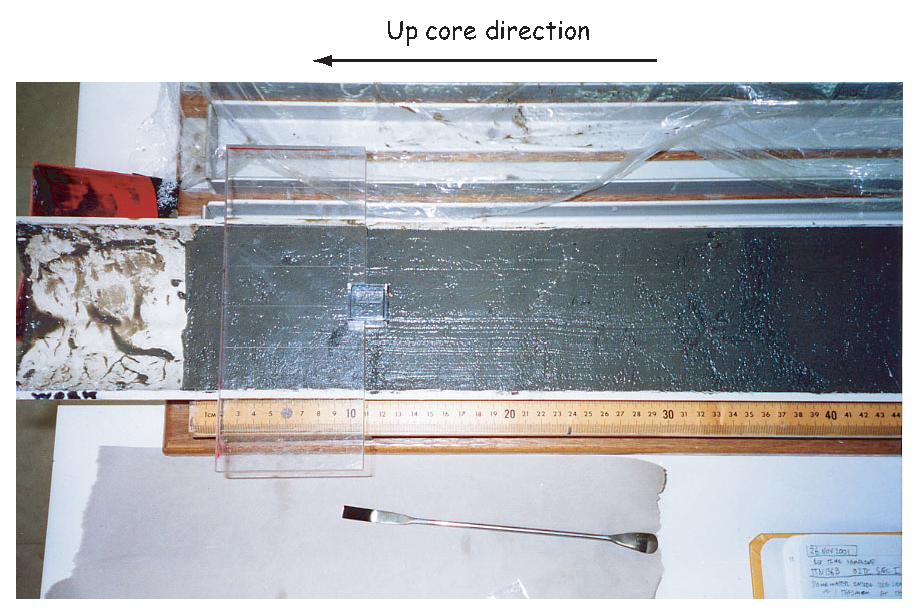
\includegraphics[width=11 cm]{EPSfiles/core.eps}
\caption{Sampling of a sediment core.  A plastic cube with a hole in it to let the air escape is pressed into the split surface of  a core.  The orientation arrow points ``up core''.  After extraction, a label with the sample name is put on. [Photo from Kurt Schwehr.] }
\label{fig:core}
\end{figure}



\item {\it Lake-bottom or sea-bottom core samples.} Numerous devices have been developed to obtain columns
of sediment from lake or sea bottom. Diameters of these coring devices are typically $\sim$10 cm
and they may be of circular or square cross section. Most such cores are azimuthally unoriented and are
assumed to penetrate the sediment vertically. Depth of penetration for ordinary piston cores is usually $<$ 20 m. 
Deep sea coring by the Deep Sea Drilling Program and its successors, the Ocean Drilling Program and the Integrated Ocean Drilling Program allow collection of 100s of meters of overlapping cores with virtually 100\% recovery. Samples for laboratory measurement are subsampled from
the sediment core (Figure~\ref{fig:core}.)

\end{enumerate} 

\begin{figure}[htb]
%\epsfxsize 12cm
%\centering \epsffile{EPSfiles/orientation.eps}
\centering  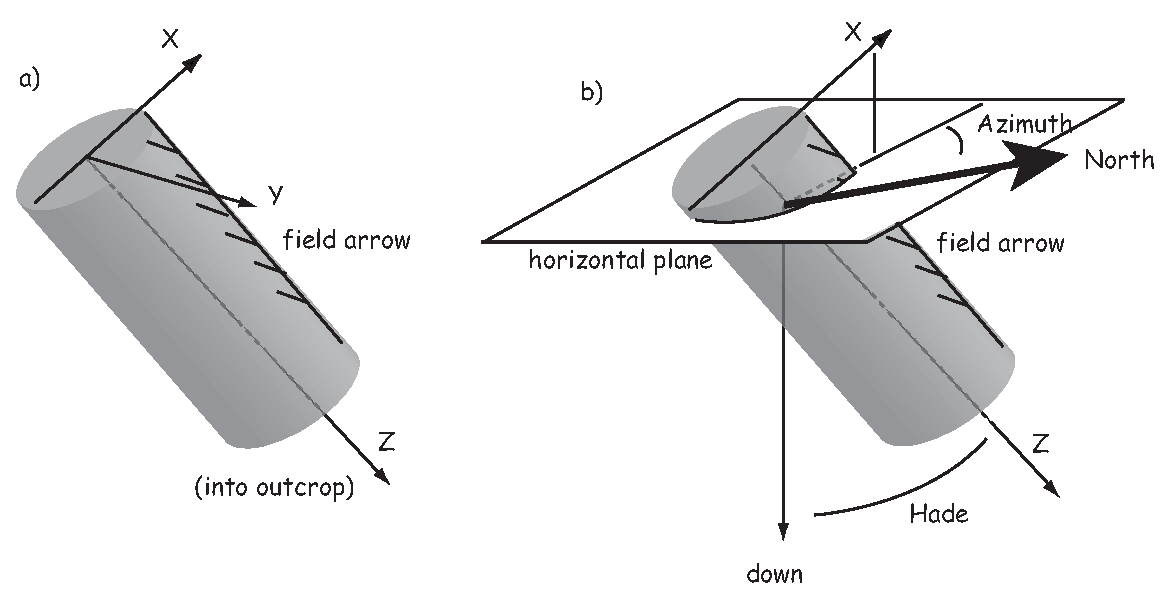
\includegraphics[width=12 cm]{EPSfiles/orientation.eps}
\caption{Orientation system for sample collected by portable core drill. a)  Schematic
representation of core sample in situ. The $Z$ axis points into outcrop; the $X $axis is perpendicular to $Z$ and is in the vertical
plane; the $Y$ axis in the  horizontal plane and is positive to the right of $X$.  b) Orientation angles for core samples. The
angles measured are the hade of the $Z$ axis (angle of $Z$ from vertical) and geographic azimuth of the
horizontal projection of the +$X$ axis measured clockwise from geographic north.   }
\label{fig:orientation}
\end{figure}



The diversity of paleomagnetic investigations and applications makes it hard to generalize about sample
collection, but there are some time-honored recommendations. One obvious recommendation is to collect
fresh, unweathered samples. Surface weathering oxidizes magnetite to hematite or iron-oxyhydroxides,
with attendant deterioration of NRM carried by magnetite and possible formation of modern CRM. Artificial
outcrops (such as road cuts) thus are preferred locations, and rapidly incising gorges provide the best
natural exposures.

Lightning strikes can produce significant secondary IRM, which can mask the primary remanence. Although partial
demagnetization in the laboratory can often erase lightning-induced IRM, the best policy is to avoid lightning-prone areas. When possible, avoid  topographic highs, especially in tropical regions. If samples
must be collected in lightning-prone areas, effects of lightning can be minimized by surveying the outcrop prior to sample collection to
find areas that have probably been struck by lightning. This is done by ``mapping'' the areas where
significant ($>5^{\circ}$) deflections of the magnetic compass occur. If a magnetic compass is passed over
an outcrop at a distance of $\sim$15 cm from the rock face while the compass is held in fixed azimuth, the
strong and inhomogeneous IRM produced by a lightning strike will cause detectable deflections of
the compass. These regions then can be avoided during sample collection.
 
\begin{figure}[htb]
%\epsfxsize 11cm
%\centering \epsffile{EPSfiles/orient.eps}
\centering  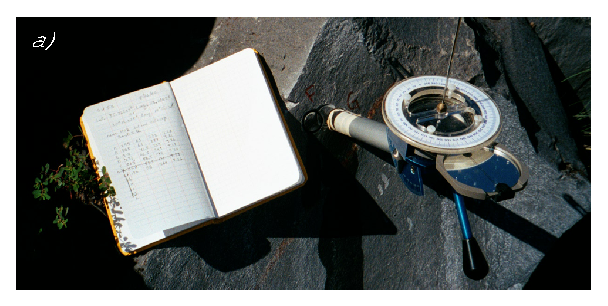
\includegraphics[width=11 cm]{EPSfiles/orient.eps}
%\centering \epsffile{EPSfiles/suncomp.eps}
\centering  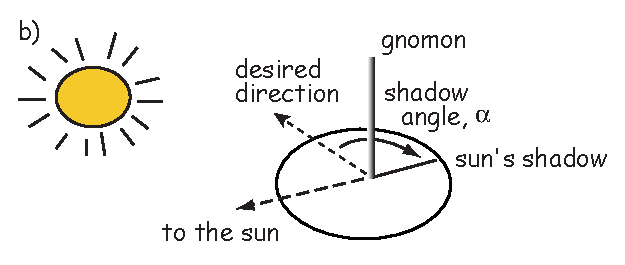
\includegraphics{EPSfiles/suncomp.eps}
\caption{a) Pomeroy orientation device in use as a sun compass.  b) Schematic of the principles of sun compass orientation.}
\label{fig:suncomp}
\end{figure}


 \subsection{Orientation in the field}
 
 In general, some direction (drill direction, strike and dip, direction of a horizontal line or even just the ``up'' direction) is measured on the sample.  This direction is here called the {\it field arrow}.  When samples are prepared into specimens for measurement, the field arrow is often replaced by a {\it lab arrow} which is frequently in some other direction.     Procedures for orienting the field arrow are varied, and no standard convention exists. However, all orientation
schemes are designed to provide an unambiguous {\it in situ} geographic orientation of each sample.    A variety of tools are used including orientation devices with magnetic and sun compasses, levels for measuring angles from the horizontal and even differential GPS devices for establishing the azimuth of a local baseline without the need for magnetic or sun compasses.  
 
If a magnetic compass is used to orient samples in the field, the preferred practice is to set the compass declination to zero.  Then, in post-processing,  the
measured azimuth must be adjusted by the local magnetic declination,
which can be calculated from a known reference 
field (IGRF or DGRF; see Chapter 2). The hade (angle from vertical down) or plunge (angle down [positive] or up [negative] from horizontal) of the sample can also be gotten using an inclinometer (either with a Pomeroy orientation device as shown in Figure~\ref{fig:drill} or with some other inclinometer, such as that on a Brunton Compass.)


Sometimes large local magnetic anomalies, for example from a strongly magnetized rock unit,  can lead to a bias in the magnetic direction that is not compensated for by the IGRF magnetic declination.  In such cases, some other means of sample orientation is required.  One relatively straightforward way is to use a 
\index{sun compass}
{\it sun compass}.  Calculation of a direction using a 
sun compass is 
more involved than for magnetic compass, however.  A dial with a vertical needle (a {\it gnomon}) is placed on the
horizontal platform shown in Figure~\ref{fig:suncomp}.  The angle ($\alpha$) that the
sun's shadow makes with the drilling direction is noted as well as the
exact time of sampling and the location of the sampling site. 
 With this information and
the aid of the Astronomical Almanac or a simple algorithm (see Appendix~\ref{app:sundec}), it is
possible to calculate the desired direction to reasonable
accuracy (the biggest cause of uncertainty is actually reading the
shadow angle!).  

Another way to avoid the deflection of the compass needle by strong local magnetic anomalies is to check the direction by sighting to known landmarks or by moving  a second magnetic  compass well away from the outcrop and  
{\it back-sighting} along the drill direction.  This is easiest by   using the sun-compass gnomon and sighting tip of the original compass as guides (see Figure~\ref{fig:backbite}).  The original magnetic compass direction (near the outcrop) can be  compared to the backsighted direction in order to detect and remove any deflection.  Of course the compass reading made with the orientation device (near outcrop) is more precise ($\sim 3^{\circ}$), but backsighting can be done with a precision of $\sim 5^{\circ}$ with care.    

\begin{figure}[htb]
%\epsfxsize 12.5cm
%\centering \epsffile{EPSfiles/backbite.eps}
\centering  \includegraphics[width=12.5 cm]{EPSfiles/backbite.eps}
\caption{Back-sighting technique using a Pomeroy orientation device and two Brunton Compasses.  One is used with the Pomeroy to measure the direction of drill and the other is used to check for deflection caused by local magnetic anomalies.}
\label{fig:backbite}
\end{figure}
\begin{figure}[h!tb]
%\epsfxsize 11cm
%\centering \epsffile{EPSfiles/gps.eps}
\centering  \includegraphics[width=11 cm]{EPSfiles/gps.eps}
\caption{ Differential GPS system for orienting paleomagnetic samples in polar regions.  Photo taken during sampling trip to the foothills of the Royal Society Ranges in Antarctica, Jan. 2004.  
}
\label{fig:gps}
\end{figure}


A new technique, developed by 
\index{Constable, C.G.}
\index{Vernon, F.L.}
C. Constable and F. Vernon at Scripps Institution of Oceanography  (see
\index{Lawrence, K.L.}
Lawrence et al. 2009) \nocite{lawrence08}  uses 
\index{differential GPS}
differential Global Positioning System (GPS) technology (see Figure~\ref{fig:gps}) to determine the azimuth of a baseline.  Two GPS receivers are attached to either end of a  one meter long non-magnetic rigid base.  The location and azimuth of the baseline can be computed from the signals detected by the two receivers.  The orientation of the baseline is transferred to the paleomagnetic samples using a laser mounted on the base which is focused on a prism attached to the orientation device used to orient the paleomagnetic samples.   The orientations derived by the differential GPS are nearly identical to those obtained by a sun compass, although it takes at least an additional half hour  and is rather awkward to transport.  Nonetheless, achieving sun-compass accuracy in orientations when the sun is unlikely to be readily available is a major breakthrough for high latitude paleomagnetic field procedures.  



\begin{figure}[htb]
%\epsfxsize 14cm
%\centering \epsffile{EPSfiles/samples.eps}
\centering  \includegraphics[width=14 cm]{EPSfiles/samples.eps}
\caption{Various types of possible specimen shapes and orientation conventions.  a) A one inch slice from a drilled core.    b) A cubic specimen of sediment sanded from a hand sample. c) A specimen (also sample) from a piston core.}
\label{fig:samples}
\end{figure}

\subsection {A note on terminology}

Samples are brought to the laboratory
 and trimmed into  standard sizes and shapes (see Figure~\ref{fig:samples}).  These sub-samples are called
 \index{paleomagnetic!specimen}
{\it paleomagnetic specimens}.  A rule of thumb about terminology is that a sample is something you take and a specimen is something you measure.   The two may be the same object, or there may be multiple specimens per sample.    A site is a single horizon or instant in time and may comprise multiple samples or may be only a single sample, depending on the application.  Multiple specimens from a single site are expected to have recorded the same geomagnetic field.    




\section{Measurement of magnetic remanence}
\label{sect:meas}

     
We measure the magnetic remanence of paleomagnetic specimens in a 
\index{magnetometer!rock}
{\it rock magnetometer}, of which there are various types.  The cheapest  are
\index{magnetometer!spinner}
 {\it spinner magnetometers} so named because
they spin the specimen to create a fluctuating electromotive force 
(emf).  The emf is
proportional to the magnetization and can be determined relative to the three
axes defined by the sample coordinate system.   The magnetization along a
given axis is measured by detecting the voltages induced by the spinning
magnetic moment within a set of pick-up coils.




Another popular way to measure the magnetization of a specimen is to use a
\index{magnetometer!cryogenic}
{\it cryogenic magnetometer}.
 These magnetometers operate 
using so-called
\index{superconducting quantum interference device}
 {\it superconducting quantum interference
devices}  (SQUIDs). In a SQUID, 
the  flux of an inserted specimen is opposed by a  
current in a loop of superconducting wire.  
The superconducting loop is constructed with a {\it weak link}
which stops superconducting at some very low current density, corresponding to some very small
quantum of flux.  Thus the flux within the loop can
change by discrete quanta.  Each incremental change is counted and the total
flux is proportional to  the magnetization along the axis of the SQUID.  
Cryogenic magnetometers are much faster and more sensitive than
spinner magnetometers, but they cost much more to buy and to operate.   

Magnetometers are used to
 measure the three components of the magnetization necessary to
define a vector (e.g., $x_1,x_2,x_3$ or equivalently $x,y,z$).  These data 
can be converted to the more common form of
$D$, $I$ and $M$  by methods described in Chapter 2. 




\section {Changing coordinate systems}


Data often must be transformed from the specimen coordinate system into, 
\index{coordinate systems!geographic}%
for example, geographic coordinates.  This can be done graphically
with a stereonet or by means of matrix manipulation.  We outline the general case for transformation of coordinates in Appendix~\ref{app:coord}.  Here we examine the specific cases of the transformation from specimen coordinates to geographic coordinates and the transformation of geographic coordinates to tilt corrected coordinates, the two most commonly used rotations in paleomagnetism.  

No matter how the sample was taken,  data in the laboratory are measured with respect to the specimen coordinate system, so all the field arrows, no matter how obtained, must be converted into the direction of the lab arrow ($x $; see example in  Figure~\ref{fig:orientation} and Figure~\ref{fig:samples}a for field drilled samples.)      Suppose we measured a magnetic moment $m$ (Figure~\ref{fig:digeo}a).  The components of $m$ in specimen coordinates are $x, y, z$ or equivalently, $x_1, x_2, x_3$.   Ordinarily, this coordinate system is at some arbitrary angle to the geographic coordinate system, but we know the azimuth and plunge ($Az, Pl$) of the lab arrow with respect to the geographic coordinate system (Figure~\ref{fig:digeo}b).   By substituting $Az$ and $Pl$ for $\phi$ and $\lambda$ into Equation~\ref{eq:aij}, the components of the direction of $m$ in geographic coordinates can be calculated.  These then can be converted back into $D, I$ and $m$ using the equations given in Chapter 2.  Note that $m$ stays the same during the transformation of coordinates.  

To correct for tilt, it is simplest to understand if this is performed as three rotations.  This is how it is done graphically with a stereonet and it is possible to do it the same way with a computer.  [It can also be done as a single rotation, which would be computationally faster, but much harder to visualize.]    First, rotate the direction of magnetic moment in specimen coordinates about a vertical axis by subtracting the dip direction from the declination of the measurement.   Then substitute $\phi=0$ and $\lambda=$ - dip into Equation~\ref{eq:aij} to bring the dip back up to horizontal.  Finally, rotate the direction  back around the vertical axis by adding the dip direction back  on to the resulting rotated declination.   

\begin{figure}[h!tb]
%\epsfxsize 12cm
%\centering \epsffile{EPSfiles/digeo.eps}
\centering  \includegraphics[width=12 cm]{EPSfiles/digeo.eps}
\caption{a) Specimen coordinates with $X_1$ being along the ``lab arrow''.  A magnetic moment $m$ was measured relative to the specimen coordinate system with components $x_1, x_2, x_3$.  The orientation of the lab arrow with respect to geographic coordinates ($X'_1 = N$) is specified by the azimuth and plunge ($Az, Pl$) of the lab arrow. }
\label{fig:digeo}
\end{figure}

\begin{figure}[p]
%\epsfxsize  11cm
%\centering \epsffile {EPSfiles/comps.eps}
\centering  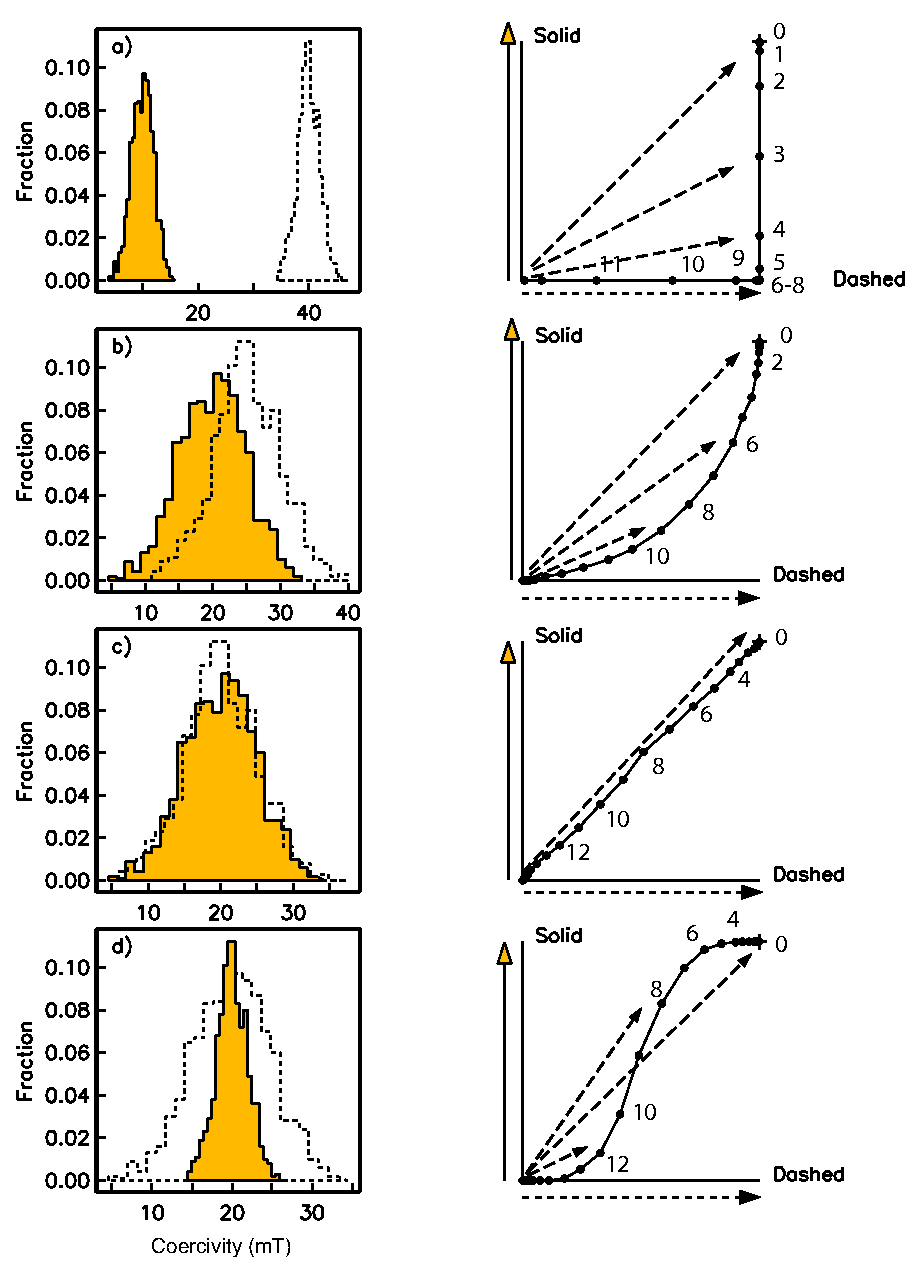
\includegraphics[width=11 cm]{EPSfiles/comps.eps}
\caption {Principle of progressive demagnetization.
Specimens with two components of magnetization (shown by heavy arrows on
the right hand side), 
with discrete coercivities (plotted as histograms to the left).
The original ``NRM'' is the sum of the two magnetic
 components and is shown as the 
+ in the diagrams to the right.
Successive demagnetization steps (numbered)  remove the component with coercivities
lower than the peak field, 
and the NRM vector changes as a result. a) The two
distributions of coercivity are completely separate.
b) The two distributions partially overlap resulting in simultaneous removal of
both components.  c) The two distributions 
completely overlap.  d) One
distribution envelopes the other.  [Figure redrawn from Tauxe, 1998.]
}
\label{fig:comps}
\end{figure}
%\clearpage

\begin{figure}[htb]
%\epsfxsize 14cm
%\epsffile {EPSfiles/zijd.eps}
\centering  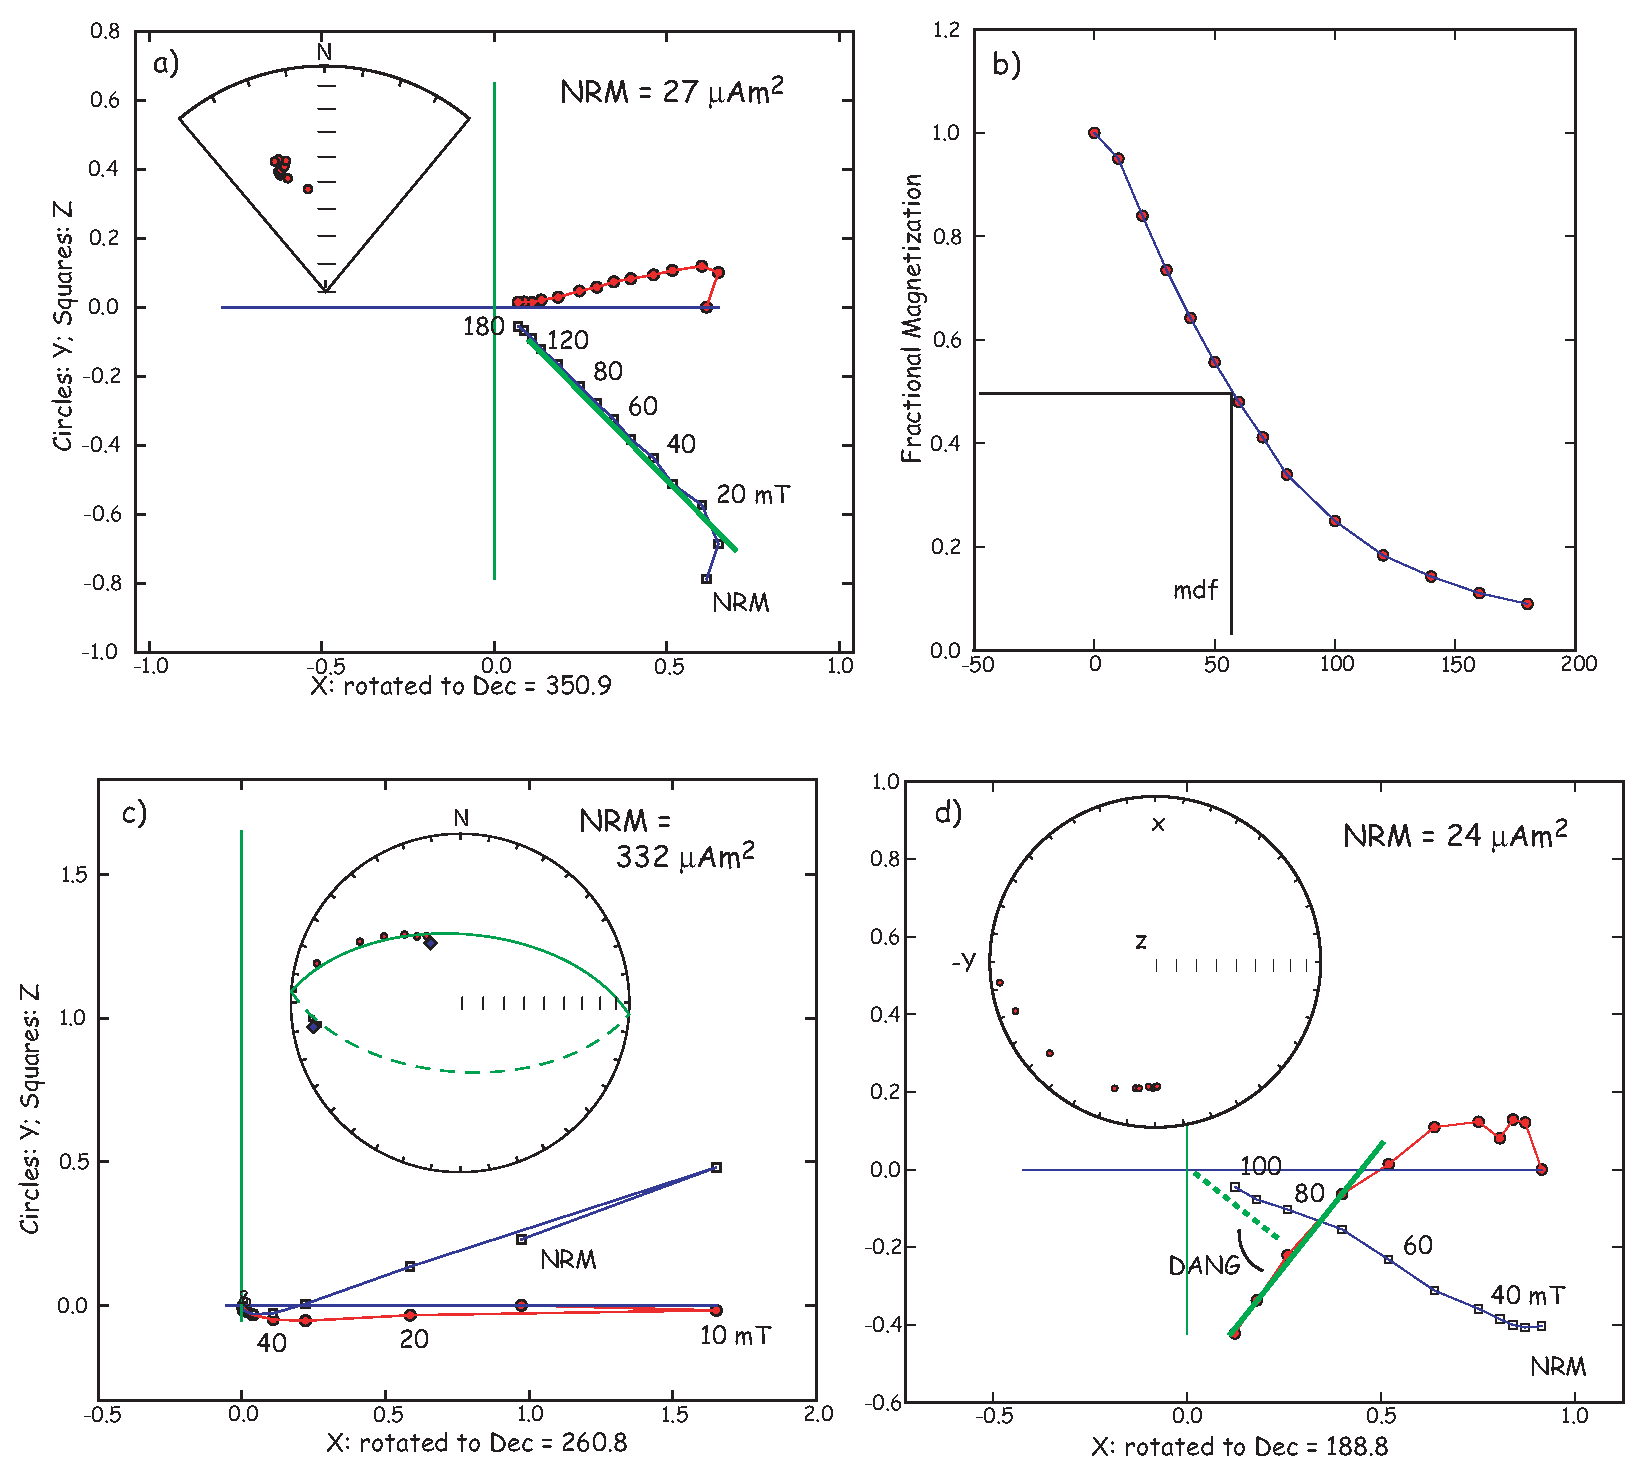
\includegraphics[width=14 cm]{EPSfiles/zijd.eps}
\caption{a) Solid (open) symbols are horizontal (vertical) projections respectively.  
 Peak alternating fields for each demagnetizing step (in mT) are indicated.  
  Inset is equal area plot of the same data.   Solid (open) symbols are projections onto the lower (upper)
hemisphere.  b) Intensity  as a function of demagnetization step.  Data from a).   
The median destructive field (mdf of Chapter 8) also shown.  c)  Specimen with  two components with overlapping stabilities.  Inset  as in a).   Best fit great circle is shown as the curve through the data (dashed portion is upper hemisphere projection). d) Data from specimen showing evidence of GRM (see Chapter 7).  During  demagnetization, the vector grows perpendicular the last demagnetization direction (-Y).  Deviation ANGle, DANG also shown.  }
\label{fig:zijd}
\end{figure}\nocite{tauxe03b} \nocite{tauxe04b} 

\clearpage


\section {Demagnetization techniques}
\label{sect:demag}


Anyone who has dealt with magnets (including magnetic tape, credit
cards, and  magnets) knows that they are delicate and  likely to 
demagnetize or change their magnetic properties if abused by heat, large magnetic fields or stress. 
Cassette tapes left on the dashboard of the car in the hot sun never sound the
same.  Credit cards that have been through the dryer may lead to acute
embarrassment at the check-out counter.
 Magnets that have been dropped, do not work as well
afterwards.  It is not difficult to imagine  that rocks that have been
left in the hot sun or buried deep in the crust (not to mention 
altered by diagenesis  or 
 bashed with hammers, drills, pick axes, etc.), may not have their
original magnetic vectors completely intact.  Because rocks often
contain
millions of tiny magnets, it is possible that some (or all) of these have
become realigned, or that they 
grew since the rock formed.  In many cases, there are
still grains that carry the original remanent vector, but there are
often populations of grains that have acquired  new components of
magnetization. The good news is that
viscous magnetizations are carried by grains with  
 lower magnetic anisotropy energies (they are 
``softer'', magnetically speaking), so  we  expect 
their contribution to be more easily randomized than
the more stable (``harder'') grains carrying the ancient remanent
magnetization. 

There are several laboratory techniques that are available for
separating various components of magnetization. 
Paleomagnetists rely on the relationship of relaxation time, coercivity, and
temperature in order to remove ({\it demagnetize}) low stability remanence
components.  The
fundamental principle that underlies demagnetization techniques is that the lower
the relaxation time $\tau$, the more likely the grain will carry a secondary
magnetization.  The basis for 
\index{demagnetization!alternating field}
{\it alternating field} (AF) demagnetization 
 is that components with short relaxation times also have low coercivities.
The basis  for
\index{demagnetization!thermal}
 {\it thermal} demagnetization is that these grains also
have low blocking temperatures.


In AF demagnetization,  an oscillating field is applied to a
paleomagnetic specimen in a null magnetic
field environment (Figure~\ref{fig:arm} in Chapter 7).  All the grain moments with
coercivities below the peak AF will track the field.  These entrained moments
will become stuck as the peak field gradually decays below the
coercivities of individual grains.   Assuming that there is a range of
coercivities in the specimen, the low stability grains will be stuck half along
one direction of the AF and half along the other direction; the net
contribution to the remanence will be zero. In practice, we
demagnetize specimens sequentially along three orthogonal axes, or
while ``tumbling'' the specimen around three axes during
demagnetization.


Thermal demagnetization exploits the relationship of relaxation time and temperature.  There will be a temperature below the Curie temperature at which the relaxation time is a few hundred seconds.  When heated to this temperature, grains with relaxation times this short will be in equilibrium with the field.  This is the {\it unblocking temperature}.  If the external field is zero, then there will be no net magnetization.  Lowering the temperature back to room temperature will result in the relaxation times growing exponentially until these moments are once again fixed.  In this way, the contribution of lower stability grains to the NRM can be randomized.  Alternatively, if there is a DC field applied during cooling, the grains whose unblocking temperatures have been exceeded will be realigned in the new field direction;  they will have acquired a partial thermal remanent magnetization (pTRM).  


We sketch the principles of progressive 
\index{demagnetization!step-wise}
(step-wise) demagnetization in
Figure~\ref{fig:comps}.  Initially, the NRM is the sum 
of two components carried by populations with different coercivities.
The distributions of coercivities are shown in the histograms to the
left in Figure~\ref{fig:comps}.  Two components of magnetization
 are shown as heavy lines
in the plots to the right.  In these examples, the two components are
orthogonal.  The sum of the two components at the start (the NRM or demagnetization step `0') is shown as a
+ on the vector plots to the right.  
After the first AF demagnetization step, the contribution
of the lowest coercivity grains has been erased and the remanence
vector moves to the position of the first dot away from the +.
  Increasing the AF in successive treatment steps (some are numbered in the diagram)
gradually eats away at  the remanence vectors (shown as dashed
arrows and dots in the plots to the right) which eventually
approach
the origin.  

There are four different sets of coercivity spectra shown in Figure~\ref{fig:comps},
each with a distinctive behavior during demagnetization.
If the two coercivity fractions are completely distinct, the
two components are clearly defined (Figure~\ref{fig:comps}a) by the
progressive demagnetization. 
If there is some overlap in the coercivity distribution of the
components the resulting demagnetization 
diagram is curved (Figure ~\ref{fig:comps}b).
If the two components completely overlap, both components are removed
simultaneously and an apparently single component demagnetization diagram 
may result (Figure~\ref{fig:comps}c). 
It is also possible for one 
coercivity spectrum to include another as shown in Figure~\ref{fig:comps}d.  Such  cases result in ``S'' shaped demagnetization curves.
 Because complete overlap actually happens in ``real''
rocks, it is desirable to perform both AF and thermal demagnetization. If the
two components overlap completely in coercivity, they might not
have overlapping  blocking temperature distributions and vice versa.   
It is unlikely that specimens from the same lithology will all have identical 
overlapping distributions, so multiple specimens can 
provide clues to the possibility of  completely 
overlapped directions in a given
specimen.


\section {Estimating directions from demagnetization data}
\label{sect:chrm}

 Now we will consider briefly the issue of what to do with the demagnetization data in terms of display and estimating a best-fit direction for various components.

The standard practice in demagnetization is to measure the NRM and then
to subject the specimen
 to a series of demagnetization steps  of increasing
severity.
The magnetization of the specimen is measured after each step.
During demagnetization,
the remanent magnetization vector will change  until 
the most stable component has been isolated, 
at which point the
vector decays in  a straight line
 to the origin.  This final component is called the 
{\it characteristic remanent magnetization} or ChRM.  





Visualizing demagnetization data is a
three-dimensional problem and therefore
difficult to plot on paper. Paleomagnetists  often rely on a set
of two projections of the vectors, one on the horizontal plane and one on the
vertical plane.  These are variously called
\index{diagrams!Zijderveld}
\index{diagrams!vector end-point}
\index{Zijderveld, J.D.A.}
Zijderveld diagrams (Zijderveld, 1967),\nocite{zijderveld67} orthogonal
projections, or vector end-point diagrams.  


 In orthogonal projections, the
 $x_1$  component is plotted versus $x_2$ (solid
symbols) in one projection,
  and $x_1$ is replotted versus Down ($x_3$) (open symbols) in
another projection.   The
paleomagnetic convention differs from the usual x-y plotting convention
because $x_3$ is on a vertical axis which is positive in the downward direction (instead of the usual positive up convention).  The choice of axis for the horizontal projection is a little more tricky.  $x_2$ is always positive to the right of $x_1$.   $x_1$ is frequently plotted along the horizontal axis and $x_2$ would then be on the vertical axis, again positive in the downward direction.  The paleomagnetic conventions make sense if one visualizes the diagram as a map view for the solid symbols and a vertical projection for the open symbols. 

Because $x_3$ gets plotted against whatever is chosen for the horizontal axis, the angle that the vertical projection makes will only be true inclination if the horizontal axis happens to be parallel to the remanence vector, i.e. directly along $x_1$.  For this reason, $x_2$ is sometimes plotted along the horizontal axis if the remanence vector is more parallel to $x_2$.    Some people choose to plot the pairs of points ($x_1,x_2$) versus $(H,x_3)$
where $H$ is the horizontal projection of the vector 
given by $\sqrt{x_1^2+x_2^2}$.  In this projection, 
sometimes called a {\it component plot}, the coordinate system changes
with every demagnetization step because $H$ almost always changes direction,
even if only slightly.  
Plotting $H$ versus $x_3$ is therefore a confusing and misleading practice. 
The primary rationale for doing so is because, in the traditional orthogonal projection where $x_3$ is plotted against $x_1$ or $x_2$, the vertical component 
reveals only an apparent inclination.  
In fact, the choice of horizontal component is arbitrary and could be deliberately chosen to be parallel to the remanence directions.   If something close to true inclination is desired, then, instead of plotting $H$ and $x_3$,
one can simply rotate the horizontal axes of the orthogonal plot such that it 
closely parallels the desired declination (Figure~\ref{fig:zijd}a,b).

 In the plots shown in Figure~\ref{fig:zijd}a,c we have rotated the remanence vector such that the $x_1$  component is parallel to the original NRM direction. 
In Figure~\ref{fig:zijd}, we show several general types of demagnetization behavior.  In 
Figure~\ref{fig:zijd}a,
the specimen has a North-Northwest and downward directed  NRM (see inset of equal area projection  in geographic coordinates.)  The direction does not change during demagnetization and the NRM is 
a single vector.       The median destructive field (from Chapter  8) is illustrated in Figure~\ref{fig:zijd}b.   
The specimen in Figure~\ref{fig:zijd}c shows a progressive change in direction from
a Westward and up directed component to a North and down
 direction.  The vector continuously changes direction to the end and no
final ``clean'' direction has been confidently isolated.  
These data are plotted on an equal area projection in the inset along with the trace of the  best-fitting plane (a great circle).
 The most stable
component probably lies somewhere near the best-fitting plane.    This specimen came from the outcrop depicted in Figure~\ref{fig:lightning} in Chapter 7 which had been hit by lightning.  The  presumptive IRM is much ``softer'' on demagnetization; the NRM is virtually erased by 40 mT, whereas the mdf of  the specimen that had not been hit by lightning is much higher (Figure~\ref{fig:zijd}a,b).  The NRM of the lightning hit specimen is  also more than an  order of magnitude stronger. 

The behavior  of the specimen shown in Figure~\ref{fig:zijd}d is again markedly different in that the intensity, after an initial smooth decrease, begins to climb again at high demagnetizing fields.  The direction deflects away from the origin towards  a direction that is orthogonal to the last axis to be demagnetized.  This behavior is typical of GRM acquisition during demagnetization (see Chapter 7).   

When specimens acquire a remanence either along the axis of the oscillating field (an ARM) or orthogonal to it (a GRM as in Figure~\ref{fig:zijd}d) they require a more complicated demagnetization regime than just along the three axes.  In the case of the parallel acquisition, a 
\index{demagnetization!double}
double demagnetization protocol works well.  In double demagnetization (e.g., 
\nocite{tauxe04}
\index{Tauxe, L.}
Tauxe et al., 2004),   a specimen is subjected to demagnetization along the three orthogonal axes, say along $+X_1,+X_2,+X_3$,  and is measured, then demagnetized along $-X_1,-X_2,-X_3$ and remeasured.  The two measurements are averaged to give an ARM free vector.  In the case of GRM,  
\index{Stephenson, A.}
Stephenson (1993) 
 \nocite{stephenson93} 
 developed a 
\index{demagnetization!GRM protocol}
triple demagnetization protocol whereby specimens are  demagnetized along $+X_1,+X_2,+X_3$  measured,
then demagnetized along $+X_2$, measured and   finally along $+X_1$ and measured. These three steps are averaged to give a GRM-free vector.   This method is a simplified but at times sufficient variation of the six step procedure described by Dankers and Zijderveld (1981). \nocite{dankers81}   GRMs have been associated with specimens that have a high anisotropy (e.g., 
\index{Stephenson, A.}
Stephenson, 1993; 
\index{Tauxe, L.}
Tauxe et al., 2004; 
\index{Potter, D.K.}
Potter and Stephenson, 2005),  or have a greigite magnetic remanence (e.g.,
\nocite{snowball97}
\index{Snowball, I.}
 Snowball, 1997).    





\section {Vector difference sum}
\label{sect:vds}
 
\index{vector difference sum}% 
An equal area projection may be the most useful way to present demagnetization data from a
specimen with several strongly overlapping remanence
 components (such as in
Figures~\ref{fig:zijd}c-d).    In order to represent the vector nature of
paleomagnetic data, it is
necessary to plot intensity information.  Intensity can be
plotted versus demagnetization step in an 
\index{intensity decay curve}%
{intensity decay curve} (Figure~\ref{fig:zijd}b).  
However, if there are several components with different
directions, the intensity decay curve cannot be used to determine,
say, the blocking temperature spectrum or mdf, because it is the vector
sum of the two components.  It is therefore
 advantageous to consider the decay curve of
\index{vector difference sum}%
the {\it vector difference sum} (VDS) of
\index{Gee, J.S.}
 Gee et al. (1993). \nocite{gee93}
 The VDS
 ``straightens out'' the various components by summing up the vector differences
at each demagnetization step, so the total magnetization is plotted, as
opposed to the resultant.    
 

\begin{figure}[htb]
%\epsfxsize 7cm
%\centering \epsffile{EPSfiles/foldtesta.eps}
\centering  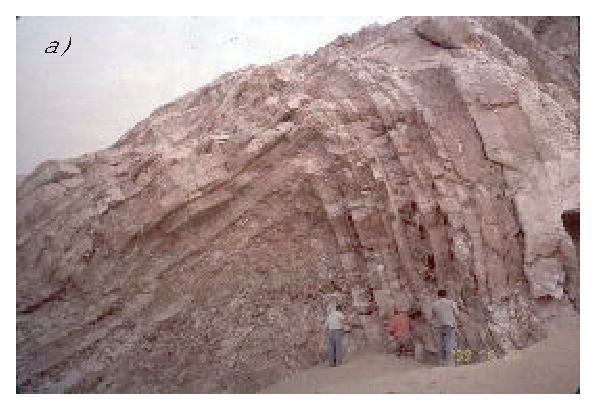
\includegraphics[width=7 cm]{EPSfiles/foldtesta.eps}
%\epsfxsize 7cm
%\centering \epsffile{EPSfiles/foldtestb.eps}
\centering  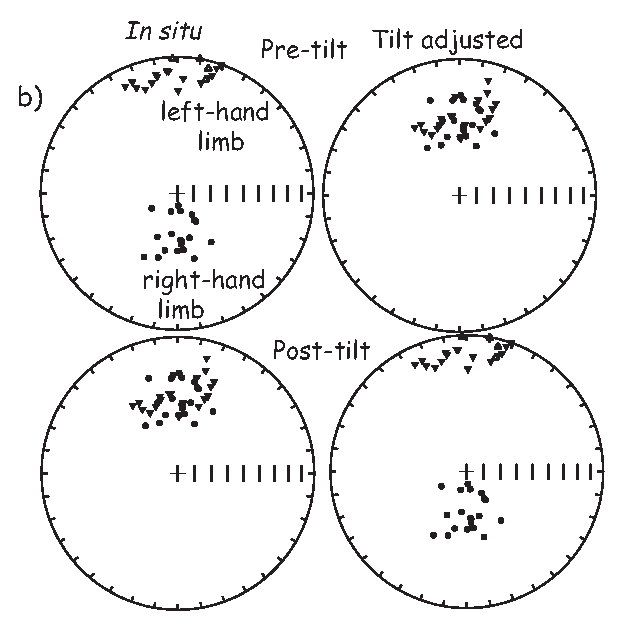
\includegraphics[width=7 cm]{EPSfiles/foldtestb.eps}
\caption{Sampling units with different bedding attitudes in the ``fold
test''. a) Example of folded beds. [Photo from G. Dupont-Nivet.]  b) Hypothetical paleomagnetic directions are shown on equal area projections before and after
adjusting for bedding tilt.  Top pair represents the case in which the grouping of paleomagnetic directions is improved after adjusting for tilt which would argue for  a pre-tilt acquisition of remanence.  Lower pair represents a post-tilt acquisition of remanence in which the grouping is worse after restoring beds to the horizontal position. }
\label{fig:fold}
\end{figure} 

  \nocite{dupont-nivet02}


\section {Best-fit lines and planes}
\label{sect:BFL}

\index{principal component analysis}%
 Orthogonal vector projections aid in   identification
of the various remanence
components in a specimen.  Demagnetization data are usually
treated using  what is known as 
\index{principal component analysis}
 {\it principal component analysis} 
\index{Kirschvink, J.}
(Kirschvink, 1980).  \nocite{kirschvink80} 
This is done by calculating the orientation tensor for the set of data and finding its eigenvectors ($\V_i$) and eigenvalues ($\tau_i$); see Appendix~\ref{app:eigen} for computational details.  
What comes out of the analysis is a best-fit line through a single component of data  as in 
Figure~\ref{fig:zijd}a,b or a best-fit plane (or great circle, if each point is given unit weight)   through multi-component data as in Figure~\ref{fig:zijd}c,d.   
\index{Kirschvink, J.}
Kirschvink [1980]  also defined the 
{\it maximum angle of deviation} or (MAD) for each of these. 

The best-fit line is given by the principal eigenvector $V_1$ and  its MAD  is given by:  

\begin{equation}
MAD = \tan^{-1}(\sqrt{(\tau_2^2+\tau_3^2})/{\tau_1}).
\label{eq:mad}
\end{equation}

\begin{figure}[h!tb]
%\epsfxsize 7cm
%\centering \epsffile{EPSfiles/congloma.eps}
\centering  \includegraphics[width=7 cm]{EPSfiles/congloma.eps}
%\epsfxsize 5cm
%\centering \epsffile{EPSfiles/conglomb.eps}
\centering  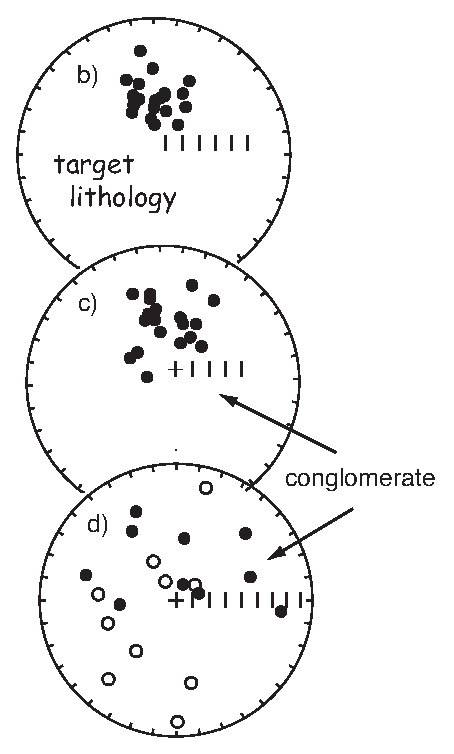
\includegraphics[width= 5 cm]{EPSfiles/conglomb.eps}
\caption {The paleomagnetic conglomerate test. a) The target lithology was involved in a catastrophic event leading to incorporation into a conglomerate bed.  Samples are taken from individual clasts.  The directions of samples from
the target lithology are shown in b) indicating that it is relatively
homogeneously magnetized.  
c) Directions from the  conglomerate clasts are also homogeneously
magnetized;
the magnetization must post-date formation of the conglomerate.  
In a positive
conglomerate test d),   the magnetization vectors
of samples from the conglomerate clasts are random.
 }
\label{fig:conglom}
\end{figure}
%\clearpage



If no unique principal direction can be isolated (as for the specimen in
Figure~\ref{fig:zijd}c-d), the eigenvector $\V_3$ associated with the least 
eigenvalue $\tau_3$ can be taken as
the pole to the best-fit plane wherein  the component of interest must lie. 
The MAD angle for the best-fit plane is given by:

\begin{equation}
MAD_{\hbox {plane}} = \tan^{-1} \sqrt { \tau_3/\tau_2 + \tau_3/\tau_1}.
\label{eq:madP}
\end{equation}

   The angle between the best-fitting line through the data and the origin is termed the 
   {\it Deviation ANGle} or DANG.  
 The line connecting the data to the origin is taken as the vector from the origin to the center of mass of the data (Equation~\ref{eq:cm}).  


\begin{figure}[htb]
%\epsfxsize 9cm
%\centering \epsffile{EPSfiles/baked.eps}
\centering  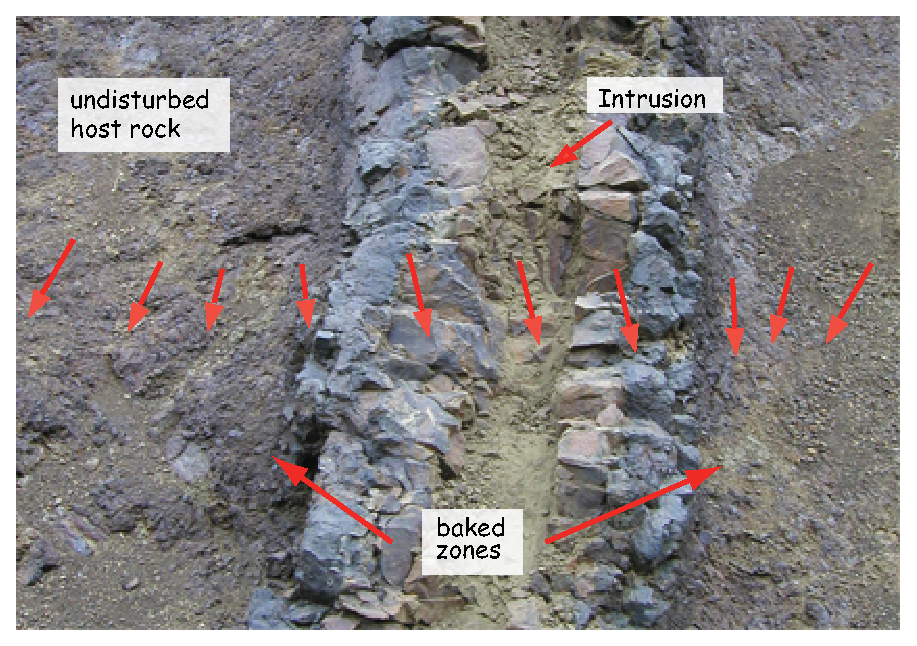
\includegraphics[width= 9 cm]{EPSfiles/baked.eps}
\caption{The baked contact test.  In a positive test, 
zones baked by the intrusion are remagnetized and have directions that
grade from that of the intrusion to that of the host rock.
If all the material is homogeneously magnetized,
then the age of the intrusion places an upper bound on the age of
magnetization.}
\label{fig:baked}
\end{figure}


\section{Field strategies}

In addition to establishing that a given rock unit
 retains a consistent magnetization, it is also important
to establish when this magnetization was acquired.  Arguments concerning the age of magnetic remanence can be
built on indirect petrographic evidence as to the relative ages of various magnetic minerals, or by evidence
based on geometric relationships in the field.
  There are two popular  field tests that require special sampling
strategies: the fold test and the conglomerate test.

The
\index{paleomagnetic tests!fold}
 {\it fold test} (also known as a {\it tilt test})  relies on the tilting or folding of the 
target geological material.
 If, for example, one wanted to establish the
antiquity of a particular set of directions, one could deliberately
sample units of like lithology, with different present attitudes 
(Figure~\ref{fig:fold}).  If the recovered directions are more tightly
grouped before  adjusting for tilt (as in the
lower left panel), then the
magnetization is likely to have been acquired after tilting.  On the other hand, if
directions become better grouped in the tilt adjusted coordinates (see upper right panel),
 one
has an argument in favor of a pre-tilt age of the magnetization.  
Methods for quantifying the tightness of grouping in various coordinate
systems will be discussed in  later chapters.


In the
\index{paleomagnetic tests!conglomerate}
 {\it conglomerate test}, lithologies that are  desirable for
paleomagnetic purposes must be found in a conglomerate bed
(Figure~\ref{fig:conglom}a).  In this
rare and happy circumstance, we can sample them and show that: 1) the
rock magnetic behavior is the same  for the conglomerate samples as
for those being used in the paleomagnetic study, 2) the directions
of the studied lithology are well grouped, (Figure~\ref{fig:conglom}b) and
3) the directions from the conglomerate clasts 
are randomly oriented (see Figure~\ref{fig:conglom}d).  If the directions of the clasts are not randomly distributed
(Figure~\ref{fig:conglom}c), 
then presumably the conglomerate clasts (and, by inference, 
the paleomagnetic samples from the studied lithology as
well) were magnetized after deposition of the conglomerate. 
We will discuss statistical methods for deciding if a set of directions
is random in later chapters.  


\index{paleomagnetic tests!baked contact}%
The {\it baked contact test} is illustrated in Figure~\ref{fig:baked}.  It
is similar to the conglomerate test in that we seek to determine whether the 
lithology in question has undergone pervasive secondary overprinting.  When
an igneous body intrudes into an existing 
{\it host rock}, it heats (or bakes) the contact zone to above the Curie temperature of the host
rock.  The baked contact immediately adjacent to the intrusion should therefore
have the same remanence direction as the intrusive unit.  This
magnetization
may be in an entirely different direction from the pre-existing host rock. The
maximum temperature reached in the baked zone decreases away from the intrusion
and remagnetization is not complete.  Thus the NRM directions of the baked zone
gradually change from that of the intrusion to that of the host rock.  Such
a condition would argue against pervasive overprinting in the  host rock that post-dated the
intrusion,  and the age of the intrusion would provide an 
upper bound on the age of remanence in the host rock.

\vskip 6pt
\noindent SUPPLEMENTAL READINGS: Collinson (1983), Chapters 8 and 9. \nocite{collinson83}

\vskip -6pt

\section{Problems}
{\parindent 0pt  \parskip 6pt

Before you start, make sure you have the most recent distribution of the {\bf PmagPy} software (see \href{http://earthref.org/PmagPy/cookbook/}{PmagPy website}) and see instructions in Problem 2 in Chapter 5 for help in accessing the data files.  Find the data files for these problems in the Essentials\_Examples/Chapter\_9 directory.    


  
{\bf Problem 1 }

The remanence vectors in the Chapter\_9 directory saved in {\it zijd\_example.csv} were measured during the 
thermal demagnetization of a specimen.  The first column is the specimen name. The second is the temperature to which the specimen was heated, before cooling in zero field.  The next columns are intensity, declination and inclination respectively for each   treatment step.  

a) Write a python program in a Jupyter notebook to make a Zijderveld diagram using python.  
 
Follow these steps:  1) Read in the data.  2) Convert the vectors to $x, y, z$.  3) Plot $x$ versus $-y$ using some solid symbol and then connect those dots with a line.  This is the horizontal projection  of the vector so $x$ should be on the horizontal axis and $-y$ should be up. (Think about this!   You are plotting a map view and Y is the East direction.  So $+y$ should be to the right of $x$.)   4) Now plot $ x $ versus $-z$.  Here again the projection is unusual because $+z$ is the down direction. Therefore it should be down.  [It is  $-z$ that is up!]    Use a different (open) symbol for these points and plot them on the same plot as your $x,y$ data.   

b) The same data were saved without headers in a file named  {\it zijd\_example.dat}.  Plot them using the program {\bf zeq.py}. [Hint:  check the help message by typing {\bf zeq.py -h} on the command line to figure out how...].  This can be done either from the command line or from within a jupyter notebook (remember that to run a command line program, you use the syntax):
\begin {verbatim}
!zeq.py -h
\end{verbatim}

Compare your answer from Problem 1a  with that produced by the PmagPy program {\bf zeq.py}.  Re-write your program until it is right; you can cheat by looking in zeq.py and the two function modules {\bf pmag.py} and {\bf pmagplotlib.py}  (see the \href{https://earthref.org/PmagPy/#zeq.py}{PmagPy Cookbook documentation}   if you have to, but make your program ``your own''.   Set the -sav and -png flags to save your figures and display them in your notebook using the Image function from IPython.display as you did in Chapter 5.  



c)     Assuming these data have already been converted to geographic coordinates $(x=N,y=E,z=V)$, what is the approximate direction (e.g. NE and up) of the low stability component
of magnetization? The high stability component of magnetization? What is
the most likely remanence carrying mineral in this specimen?   Thinking about what you learned about VRM in Chapter 7, for the low stability component to be a VRM acquired over the last million years,  at what temperature would the rock have to have been held to acquire this component viscously over a million years?  


c) Run  {\bf zeq.py} again, this time setting the -beg and -end flags to calculate best-fit lines through the two components and a great circle through all the data except the NRM and last steps.  Display these new images in your notebook.  In a markdown code block explain which interpretation makes the most sense?  



{\bf Problem 2 }

a) Use the program {\bf sundec.py}  from the command line to estimate what the drilling azimuth was using the following sun compass information:   You are located at 35$^{\circ}$ N and 33$^{\circ}$ E.  The local
time is three hours ahead of Universal Time, so we subtract -3 from local time.  The shadow angle for the
drilling direction was 68$^{\circ}$ measured at 16:09 on May 23, 1994.

b) Now use the dosundec() function from the pmagpy.pmag  module to do the same thing.  

{\bf Problem 3}
% problem 4.2 from Butler 1992:

a) The direction of NRM  for these problem is given in geographic coordinates along with the
attitude of dipping strata from which the site was collected:    

D = 336$^{\circ}$, I = -2$^{\circ}$, bedding dip = 41$^{\circ}$, dip direction = 351 $^{\circ}$.  

Plot the NRM direction on an equal-area
projection (see Appendix~\ref{app:eqarea}).   Then using the procedures outlined in Appendix~\ref{app:eqtilt} (or slight modifications thereof), determine
the ``structurally corrected'' direction of NRM that results from restoring the strata to horizontal.

Check your answer with the program {\bf di_tilt.py}

b) Now try the same problem using the pmagpy.pmag function dotilt() in a Jupyter notebook.   



{\bf Problem 4}
%Problem 4.3 from Butler 1992.

Now consider a more complex situation in which a paleomagnetic site has been collected from the
limb of a plunging fold. On the east limb of a plunging anticline, a direction of NRM is found to be
I = 33$^{\circ}$, D = 309$^{\circ}$. The bedding attitude of the collection site is dip = 29$^{\circ}$, strike = 210$^{\circ}$ (dip direction = 120$^{\circ}$, and the pole to bedding is azimuth = 300$^{\circ}$, inclination = 61$^{\circ}$). The trend and plunge of the
anticlinal axis are trend = 170$^{\circ}$, plunge = 20$^{\circ}$. Determine the direction of NRM from this site following
structural correction. To do this, first correct the NRM direction (and the pole to bedding) for the
plunge of the anticline. Rotate the fold axis to horizontal first. Then complete the structural correction of the NRM direction by restoring
the bedding (corrected for plunge) to horizontal.   Use the function {\bf pmag.dotilt() } in the {\bf PmagPy} package to do your rotations in an Jupyter notebook.    






{\bf Problem 5}  

Write a python program  to convert
$D=8.1, I=45.2$  into geographic and tilt adjusted coordinates. Use the geographic coordinates as input to the tilt correction program.   The
orientation of the laboratory arrow on the specimen was: azimuth = 347$^{\circ}$;
plunge = 27$^{\circ}$.  The  strike was 135$^{\circ}$ and the dip was 21$^{\circ}$.
(NB: the convention is that the dip direction is to the ``right'' of 
the strike).   For this it would be handy to use the {\bf numpy} module which allows arrays, instead of simple lists.  To make an array $A$ of elements $ a_{ij}$:

$$
{\pmatrix{
 a_{11}&a_{12}&a_{13}\cr
 a_{21}&a_{22}&a_{23}\cr
 a_{31}&a_{32}&a_{33}\cr
}},
$$


\noindent the command would be:

\begin{verbatim}
import numpy as np
A=np.array([[a11,a12,a13],[a21,a22,a23],[a31,a32,a33]])
\end{verbatim}

The import command can be put at the beginning of the program as always.    Use your programs to convert direction to cartesian coordinates and back again.  

Compare your answer to the one given by {\bf di\_geo.py} and {\bf di\_tilt.py} that are callable from the command line in an interactive mode.    Rewrite your code until you have it right.    NB: {\bf  di\_tilt.py}  uses dip and dip direction instead of strike and dip.  These are completely interchangeable, but dip and dip direction is unique, while strike and dip requires some convention like ``dip to right of strike'').   


\begin{figure}[h!tb]
\centering  \includegraphics[width= 14 cm]{EPSfiles/NS034.eps}
\caption{Paleomagnetic site NS034. a) Photo of the ``red'' team.  b) Photo showing sample holes with labels. The picture was taken in an easterly direction (see look direction in notebook page.)   c) Page from the notebook.  }
\label{fig:ns34}
\end{figure}


{\bf Problem 6}



 An intrepid group called ``the red team'' sampled a lava flow on Bastille day in 2006.  The team, the sampling sites and the notebook page are shown in Figure~\ref{fig:ns34}a,b and c respectively. 
In this problem we will look at some real data collected from this lava flow.  


a) Make a  new directory in your homework directory for this problem.   Do not include spaces in the directory name!
Run the {\bf Pmag GUI} graphical user interface by typing {\bf pmag\_gui.py} on the command line.  [Note that PC users may have to omit the .py termination.]  This problem does not use the Jupyter notebook!

Change directories into your new homework directory.  

b) Convert your data files to the MagIC format.   The measurements were made in the SIO paleomagnetic laboratory in the SIO lab format.  Specimens were demagnetized using the AF and thermal methods and the data are in the Chapter\_9 directory, named ns\_a.mag and ns\_t.mag respectively.  

\begin{itemize}
\item  Click on the button labeled `1. convert magnetometer files....'  and choose the `SIO format' before clicking on `Import file'.   
\item Click on `add'  and select ns\_a.mag to start.  Check the `AF Demag' box.  If you open the file you will see that the specimen names have the format:  ns034a1.   The terminal number distinguishes this from the sample, ns034a and the terminal letter distinguishes the sample from the site, ns034.  So choose the number of terminal characters....  to be `1'.  The default sample-site naming convention of XXXXY is already correct.  Now fill in the Location name to be `North Shore Volcanics' and click on `OK' at the bottom of the page.  
\item  Repeat this procedure for the thermal demagnetization data.  Be sure to click on the `Thermal (includes thellier but not trm)' button instead of AF Demag.  
\item After clicking on `OK', select `Next step'  and click on 	`OK'  to combine both measurement files into a single file.  
\item Skip the panel `Step 3:' by clicking on `OK'  to complete the conversion step.   
\end{itemize}

c)  Click on the button labelled `2. Calculate the geographic/tilt-corrected directions'.   Here you could fill out the form using the notebook information in Figure~\ref{fig:ns34}.  But someone has typed in all the data you need for you.  They are in the `Orientation file' named `orient.txt' in the Chapter\_9 directory.  
\begin{itemize}
\item Click on the button `Import Orientation File' and select that file.  This should fill in the most of the information for you.   Note that the red team's convention was to mark a sample with a $\sim$ if it broke off before orientation and to put the method code `SO-GT5' in the magic\_method\_codes column.   All  ``sample\_flag''s  are set to 'g'  (good) by default.  
\item Click on `Save Orientation File' and then `Calculate Sample Orientations'.   
These samples were oriented with a Pomeroy orientation device, so, select the first option under orientation convention.  
\item The magnetic declination of the compass was set to 0 (notebook entry says ``MagDec set to zero''.), so we need to correct all the information for magnetic declination.  Select ``Use the IGRF value at the lat/long and date supplied'' option. 
\item You will need to supply the hours to subtract from local time to get to GMT here because all the sampling times were in local time.  The entry in the notebook page says that GMT is five hours ahead of local time, so enter ``-5'' here. Click on 'OK'. 
\item  You can enter a number of sampling codes.  Here, select field drilling,  location with GPS, Pomeroy orientation device  options.   
\item  There is only one bedding plane estimate, so skip the bedding averaging option.
\end{itemize}


d) Look at the demagnetization data. 

\begin{itemize}
\item Click on the 	`Demag GUI' button.  You should have a panel of plots including a  Zijderveld plot, an equal area projection with all the demagnetization directions, a intensity decay curve, and a blank site level equal area projection.    
\item You will see a list of data to the left.   You can toggle the orientation from geographic to specimen or stratigraphic (tilt corrected) by choosing the coordinate system.   You can also change the declination for the horizontal axis of the Zijderveld diagram with the Zijderveld plot pull down menu.  The default is to rotate it to the NRM direction.    
\item  Calculate the best fit direction for this specimen by selecting data from the second demagnetization step to the end in the `bounds' drop down menus at the top left of the panel.   Choose the default to calculate a best-fit line by simply leaving the `specimen man type set to `line'.    You will see the data re-plotted with the best-fit line.   Save the interpretation by clicking on the `save' button.  
\item Step through all the data until you have interpreted all the specimens.   Notice how each interpretation shows up in the site window.  
\item  Under the 'File' menu, select `Save MagIC pmag tables'.  Use the default age of 1100 Ma for these rocks.  Then click on `OK'. 
\item Exit the program by  selecting the `Quit Demag-gui' option under the 'File' menu.  
\end{itemize}


e) Explore the MagIC database tables that you have created. 

\begin{itemize}
\item  Look at  the chapter on the MagIC database and file formats in the \href{http://earthref.org/PmagPy/}{PmagPy cookbook}.  
\item Click on the Pmag GUI's button `3. fill Earth-Ref data' and verify the relationship of the specimens to the samples.  Click on `Save and continue'.  
\item Repeat this for Step 2. 
\item For Step 3, you must insure that site `s034' belongs to `North Shore Volcanics', which you must add with the `Add a new location' button.  Then click on the cell below locations and select that.    
\item These were extrusive igneous rocks, so select those options for the site\_class column.
\item find `Basalt' under the site\_lithology column and `Lava Flow' for site\_type.  
\item Then click on `Save and continue.  
\item Step 4 allows you to verify that everything you have done was propagated correctly to the site level.  Click on `Save and continue'.   
\item For step 5, you must let the program know what type of location these samples were taken from, so select `Outcrop' under that column.  Then select `Save and continue'.   
\item Step 6 deals with ages.   Fill in stratigraphic correlation for the geochronology method (GM-CC-STRAT), Ga for the age\_unit and 1.1 for the age.  
\item Click on `Save and continue' to finish.  
\end{itemize}

You can explore your handiwork by looking at the files created in your homework directory with Excel or some other spreadsheet program.   





